\documentclass[dvipdfmx,autodetect-engine, unicode, 10pt, aspectratio=169]{beamer}

% \documentclass[dvipdfmx,autodetect-engine]{jsarticle}
% \usepackage{luatexja}% 日本語
% \usepackage[haranoaji,deluxe]{luatexja-preset}% フォント指定
\renewcommand{\kanjifamilydefault}{\gtdefault}% 既定をゴシック体に

\usetheme[progressbar=frametitle]{metropolis}
\usepackage{appendixnumberbeamer}
\usepackage{booktabs}
\usepackage[scale=2]{ccicons}
\usepackage{pgfplots}
\usepgfplotslibrary{dateplot}
\usepackage{xspace}
\newcommand{\themename}{\textbf{\textsc{metropolis}}\xspace}
\usepackage{adjustbox}
\usepackage{caption}
\captionsetup[figure]{font=tiny}
\usepackage{fancyvrb} % verbatim replacement that allows latex
\usepackage{listings} % Setting for Code block
\usepackage{bm} % for Bold font in Math \bm

\title{多変量解析}
\subtitle{証券アナリスト}
% \date{\today}
\date{}
\author{Takayuki Suzuki}
\institute{This is institude of the author}

\begin{document}

\maketitle


\begin{frame}{多変量解析目標}
    線形代数(ベクトルと行列)では、「理解する」と「計算できる」が有る。 
    \begin{itemize}
        \item 主成分分析の行列計算との対応
        \item 主成分分析の主成分ベクトルの意味が説明できる
        \item 主成分得点が計算できる
        \item 因子分析と主成分分析の違いが説明できる
        \item バリマックス回転?プロマックス回転?
        \item 判別分析、クラスター分析、マハラノビス距離などの用語を知っている
    \end{itemize}
    計算できる必要があるのは、2x2の固有方程式から固有ベクトルを計算すること \\
    および対角化、そして、関数を成分とするベクトルの微分表記、計算ができること。 \\
\end{frame}

\begin{frame}{出る問題}
    結局、例の、水準(パラレルシフト)、傾き、曲率の問題に落ちる。\\
    この問題について、主成分分析にフォーカスして解説する。
    例えば、水準はたいていの場合第一主成分だが、なぜ第一主成分なのか?など。
\end{frame}

\begin{frame}{主成分分析}
    \small
    多変数からなるデータを分析する手法。\\
    データを分析するとき、変数同士に相関が無い方が分析しやすい。  \\
    また、データの変動に影響が有る変数の順番が分かっていた方が分析しやすい。\\
    しかし、一般的にデータは変数同士は相関があるし、どの変数が最も影響があるか、明らかではない。\\
    主成分分析を行うと、1.互いに独立で、2.最も影響がある変数から順番に、新しい変数を作ることができる。

    \begin{minipage}{0.45\linewidth}\scriptsize
        右は、主成分分析のイメージ。
        x,yの二つの変数のデータから、新しい軸(茶軸)を作る。\\
        元のデータは、x,yで表現されると、相関がある。(斜めの傾向が見える)\\
        しかし、新しい軸で見ると、相関が無いデータになる。\\
        しかも、最も変動が大きい方向が第一主軸となっている。
    \end{minipage}
    \begin{minipage}{0.45\linewidth}
        \begin{figure}[h]
        \centering
            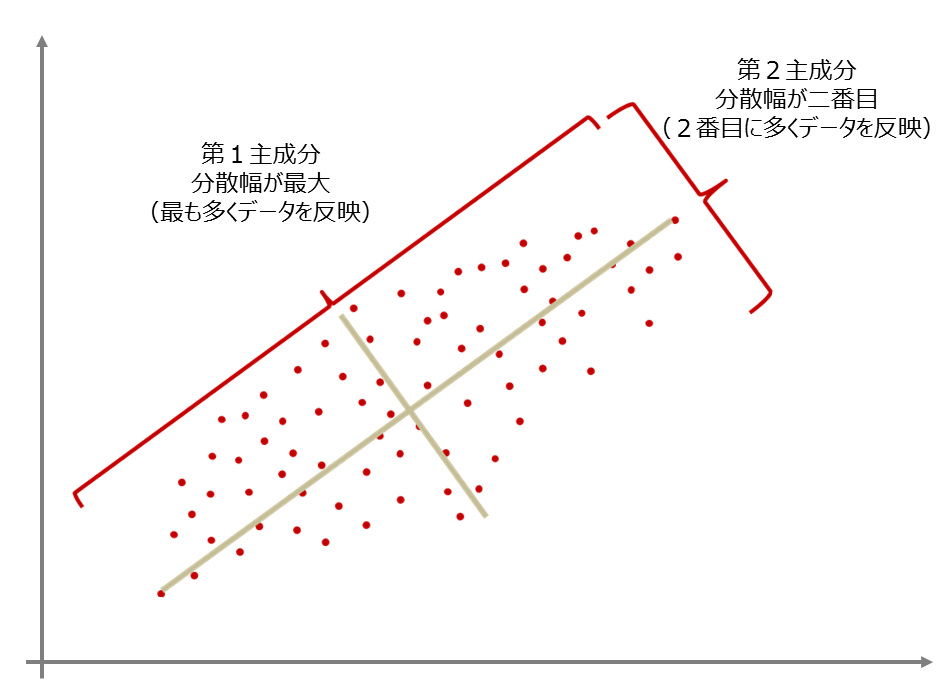
\includegraphics[width=0.9\textwidth]{PCA.png}
        \caption*{\tiny https://www.intage.co.jp/glossary/401/}
        \label{fig:mesh1}
        \end{figure}
    \end{minipage}
\end{frame}

\begin{frame}{主成分分析の計算方法}
    主成分分析は、データをよく表現する新しい変数をt来ること。どうやって作る?\\
    ⇒ 元の変数の分散共分散行列の固有値よ固有ベクトルを求めればよい (覚える)\\
    例えば、ある2変数$x_1, x_2$からなるデータが有って、それぞれの変数の分散が$\sigma_{x_1}=4, \sigma_{x_2}=7$, 共分散が$\text{cov}(x_1, x_2)=2, \text{cov}(x_2, x_1)=2$であったとき(共分散は順番が変わっても同一であるから、分散共分散行列は常に対称行列である)、これを主成分分析するには、\\
    $
        \text{分散共分散行列} = 
            \begin{bmatrix}
                4 && 2 \\
                2 && 7
            \end{bmatrix}
    $の固有値、固有ベクトルを求めればよい。前章の手順に従い、計算すると、固有値は$\lambda = 3, 8$, 対応する固有ベクトルは\\
    $\bm{w}_1 = \begin{bmatrix}
        2/\sqrt{3} \\ -1/\sqrt{3}
    \end{bmatrix}$
    および
    $\bm{w}_2 = \begin{bmatrix}
        1/\sqrt{3} \\ 2/\sqrt{3}
    \end{bmatrix}$
    であることが分かる(計算せよ)\\
    絶対値が大きい固有値8に対応するベクトル$\bm{w}_2$が、第一主軸で、固有値3に対応するベクトル$\bm{w}_1$が、第二主軸である。
\end{frame}

\begin{frame}{主成分得点}
    この主軸はどのように使うか?\\
    あるサンプルA(サンプルというのは、データの中の一点のこと)を考える。
    $A\sim \bm{x}_A = (x_1, x_2) = (3, 2)$というデータが有ったとする。このデータは、新しい軸では\\
    \begin{align*}
        A\sim \bm{x}'_A = (x'_1, x'_2) &= (\text{Aの第一主軸への射影成分}, \text{Aの第二主軸への射影成分}) \\
        & = (w_1\cdot \bm{x}_a, \hspace{5pt}  w_2 \cdot \bm{x}_a) \\
        &= \bm{P}\bm{x}_A \\
        & = \begin{bmatrix}
            \frac{8}{\sqrt{3}} \\ \frac{1}{\sqrt{3}}
        \end{bmatrix}
        \\&\footnotesize \text{ただし、$\bm{P}$は固有ベクトルを並べた行列}
    \end{align*}
    つまり、固有ベクトルとの内積を取れば求められる。内積は正射影ということもある。(行列Pを掛けるともいえる)\\
    こうして求めた新しい軸での値$(x'_1, x'_2)$のことを、主成分得点という。\\
    主成分得点から、元のデータを再現する方法は、計算できるようにしておく。
    
\end{frame}

\begin{frame}{寄与率}
    主成分のは、それぞれ寄与率というものがある。\\
    データの分散のどの程度が、どの主成分で計算できるか、を示す。\\
    それぞれの主軸の寄与率は、各主軸に対応する固有値を、すべての固有値の和で割ることで求められる。
\end{frame}

\end{document}
